\documentclass[tikz,border=2pt]{standalone}
\usepackage{amsmath}
\usetikzlibrary{arrows.meta}
\begin{document}
% Closure: the template power(e) returns b -> b^e. The calls power(2) and power(3) give the closures
% square and cube, each retaining its own e; square(5) = 25 and cube(4) = 64 (Section 1.2).
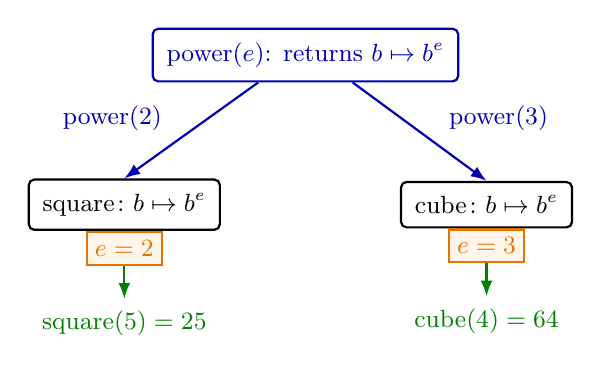
\begin{tikzpicture}[font=\small, >={Latex[length=2mm]},
  box/.style={draw, thick, rounded corners=2pt, inner sep=5pt},
  tag/.style={draw, orange!90!black, thick, fill=orange!8, inner sep=3pt}]
  \node[box, blue!70!black] (tpl) at (0,0) {$\operatorname{power}(e)$: returns $b\mapsto b^{e}$};
  \node[box] (sq) at (-2.3,-1.9) {$\operatorname{square}\colon b\mapsto b^{e}$};
  \node[box] (cu) at (2.3,-1.9) {$\operatorname{cube}\colon b\mapsto b^{e}$};
  \node[tag, anchor=north] (e2) at (sq.south) {$e=2$};
  \node[tag, anchor=north] (e3) at (cu.south) {$e=3$};
  \draw[->, thick, blue!70!black] (tpl.south) ++(-0.6,0) -- (sq.north);
  \node[blue!70!black, anchor=east] at (-1.7,-0.8) {$\operatorname{power}(2)$};
  \draw[->, thick, blue!70!black] (tpl.south) ++(0.6,0) -- (cu.north);
  \node[blue!70!black, anchor=west] at (1.7,-0.8) {$\operatorname{power}(3)$};
  \node[green!50!black, anchor=north] at ([yshift=-0.45cm]e2.south) {$\operatorname{square}(5)=25$};
  \node[green!50!black, anchor=north] at ([yshift=-0.45cm]e3.south) {$\operatorname{cube}(4)=64$};
  \draw[->, thick, green!50!black] (e2.south) -- ++(0,-0.42);
  \draw[->, thick, green!50!black] (e3.south) -- ++(0,-0.42);
\end{tikzpicture}
\end{document}
